\section{System design}
Our scatterometer (detailed in Figures \ref{fig:cad} and \ref{fig:light_path}) consists of two mutually coherent, collimated beams of wavelength 532 nm separated vertically by a small angle of approximately $4^\circ$ (assumed to be within the memory effect range for materials of interest). Both beams are attached to a stage that rotates the beams azimuthally about a scattering sample located on the stage's rotation axis. The intensity of scattered light is measured by a stationary camera as the beams are swept through a range of approximately $180^\circ$. The correlation of both beams' speckle images at a given azimuthal angle is proportional to the scattering phase function as a function of angle.

There are three primary components for acquisition. The first is the acquisition camera which we use to record speckle images. The second is the illuminator assembly which adjusts the angular illuminator separation and the azimuthal illumination direction relative to the acquisition camera. The third is the sample assembly which orients and positions the sample such that it is located on the azimuthal rotation axis of the illuminator assembly and maximal light is scattered towards the acquisition camera.
\begin{figure}
    \centering
    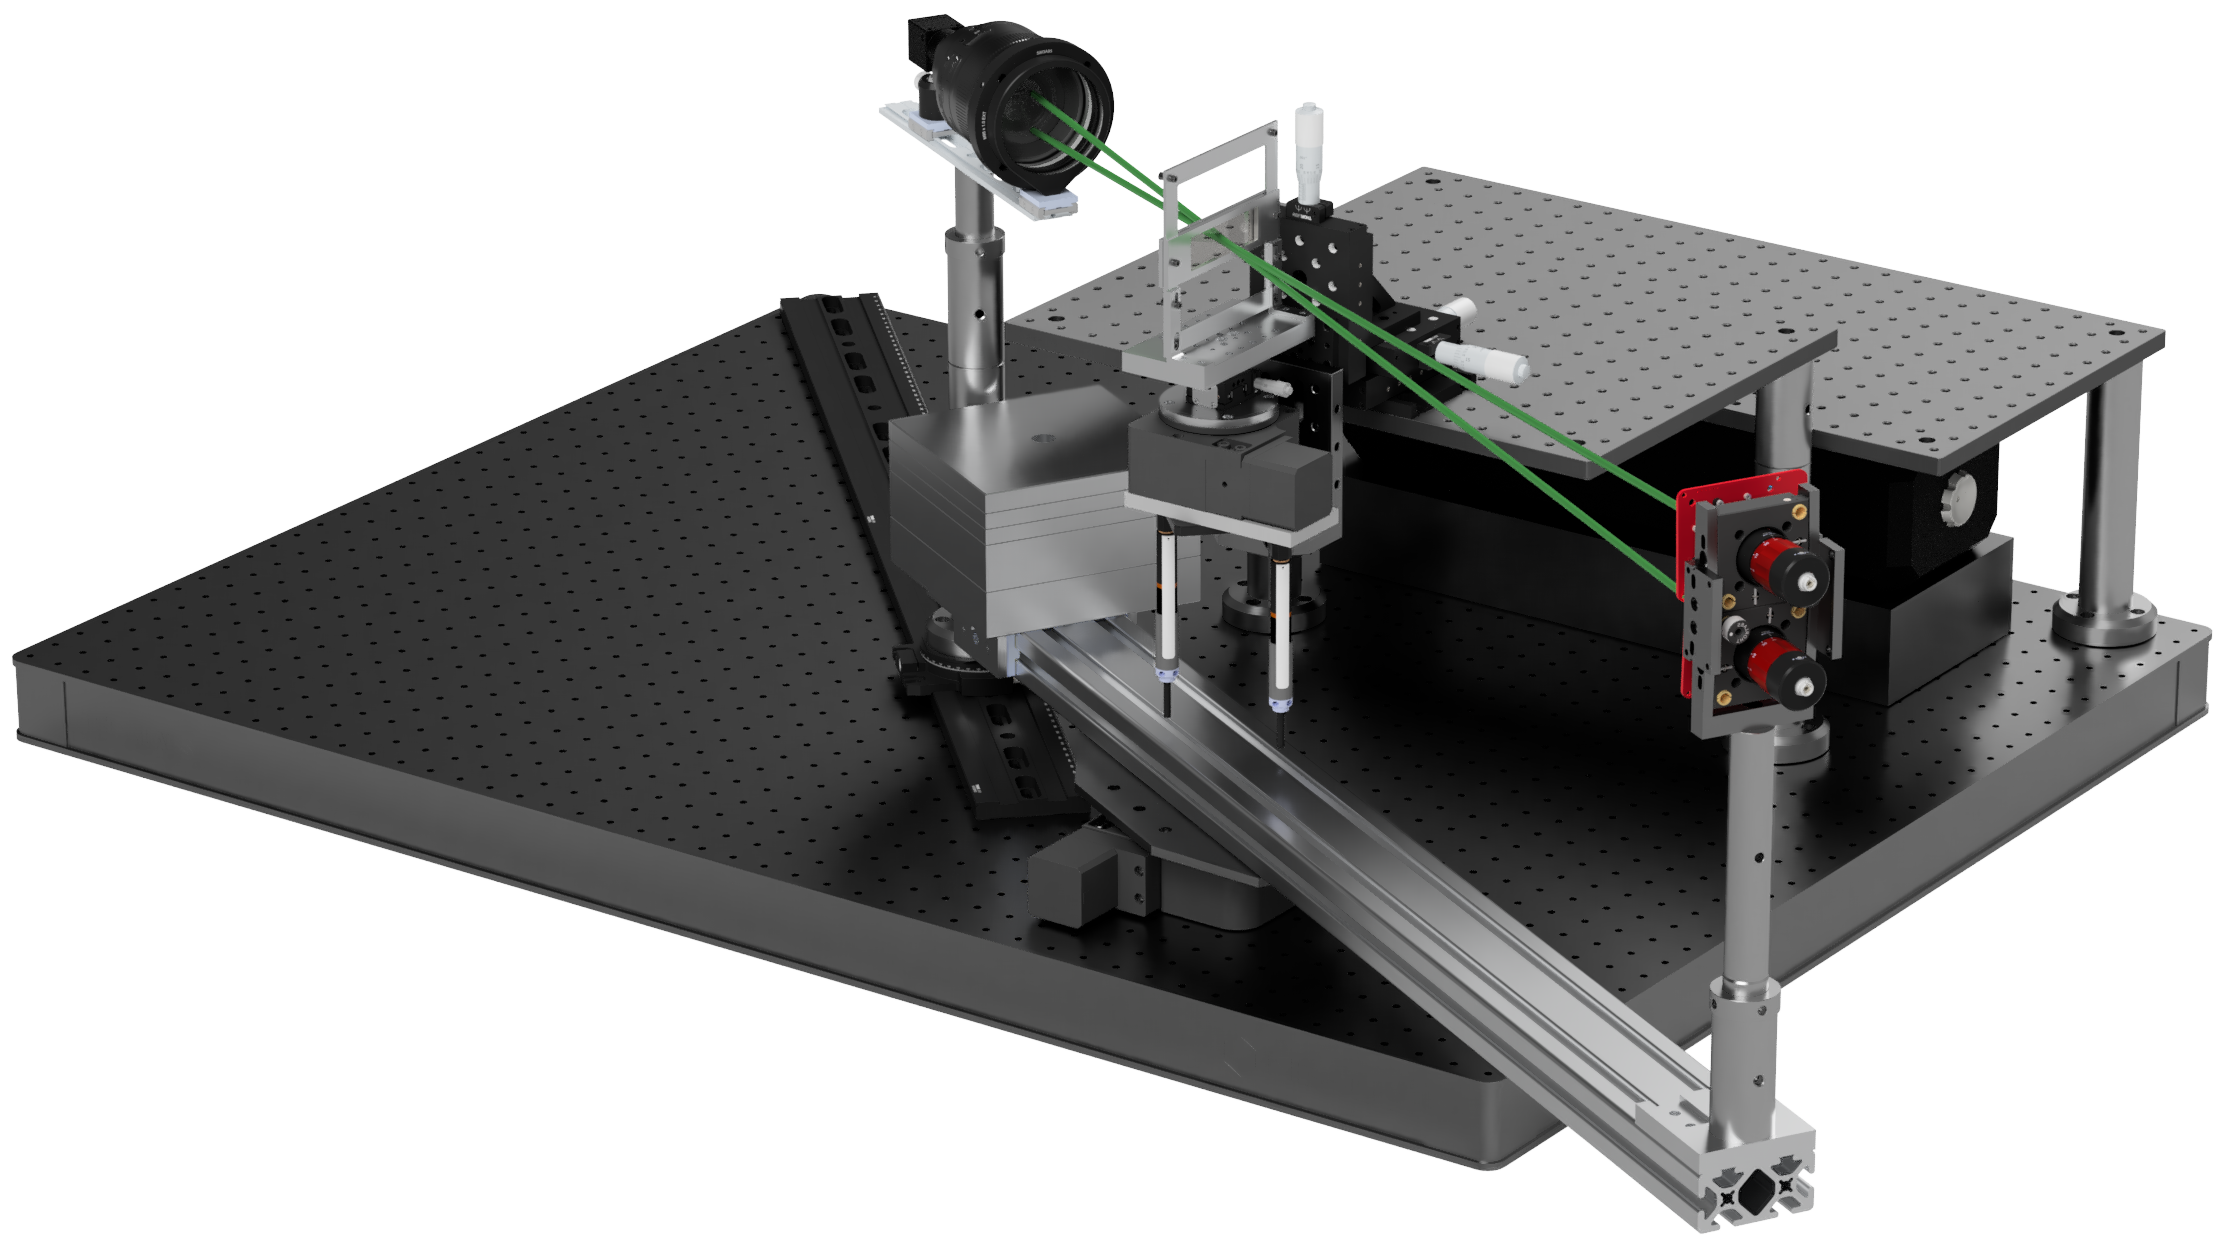
\includegraphics[width=0.75\textwidth]{figures/setup.png}
    \caption{CAD rendering of speckle correlation scatterometer}
    \label{fig:cad}
\end{figure}

\begin{figure}
    \centering
    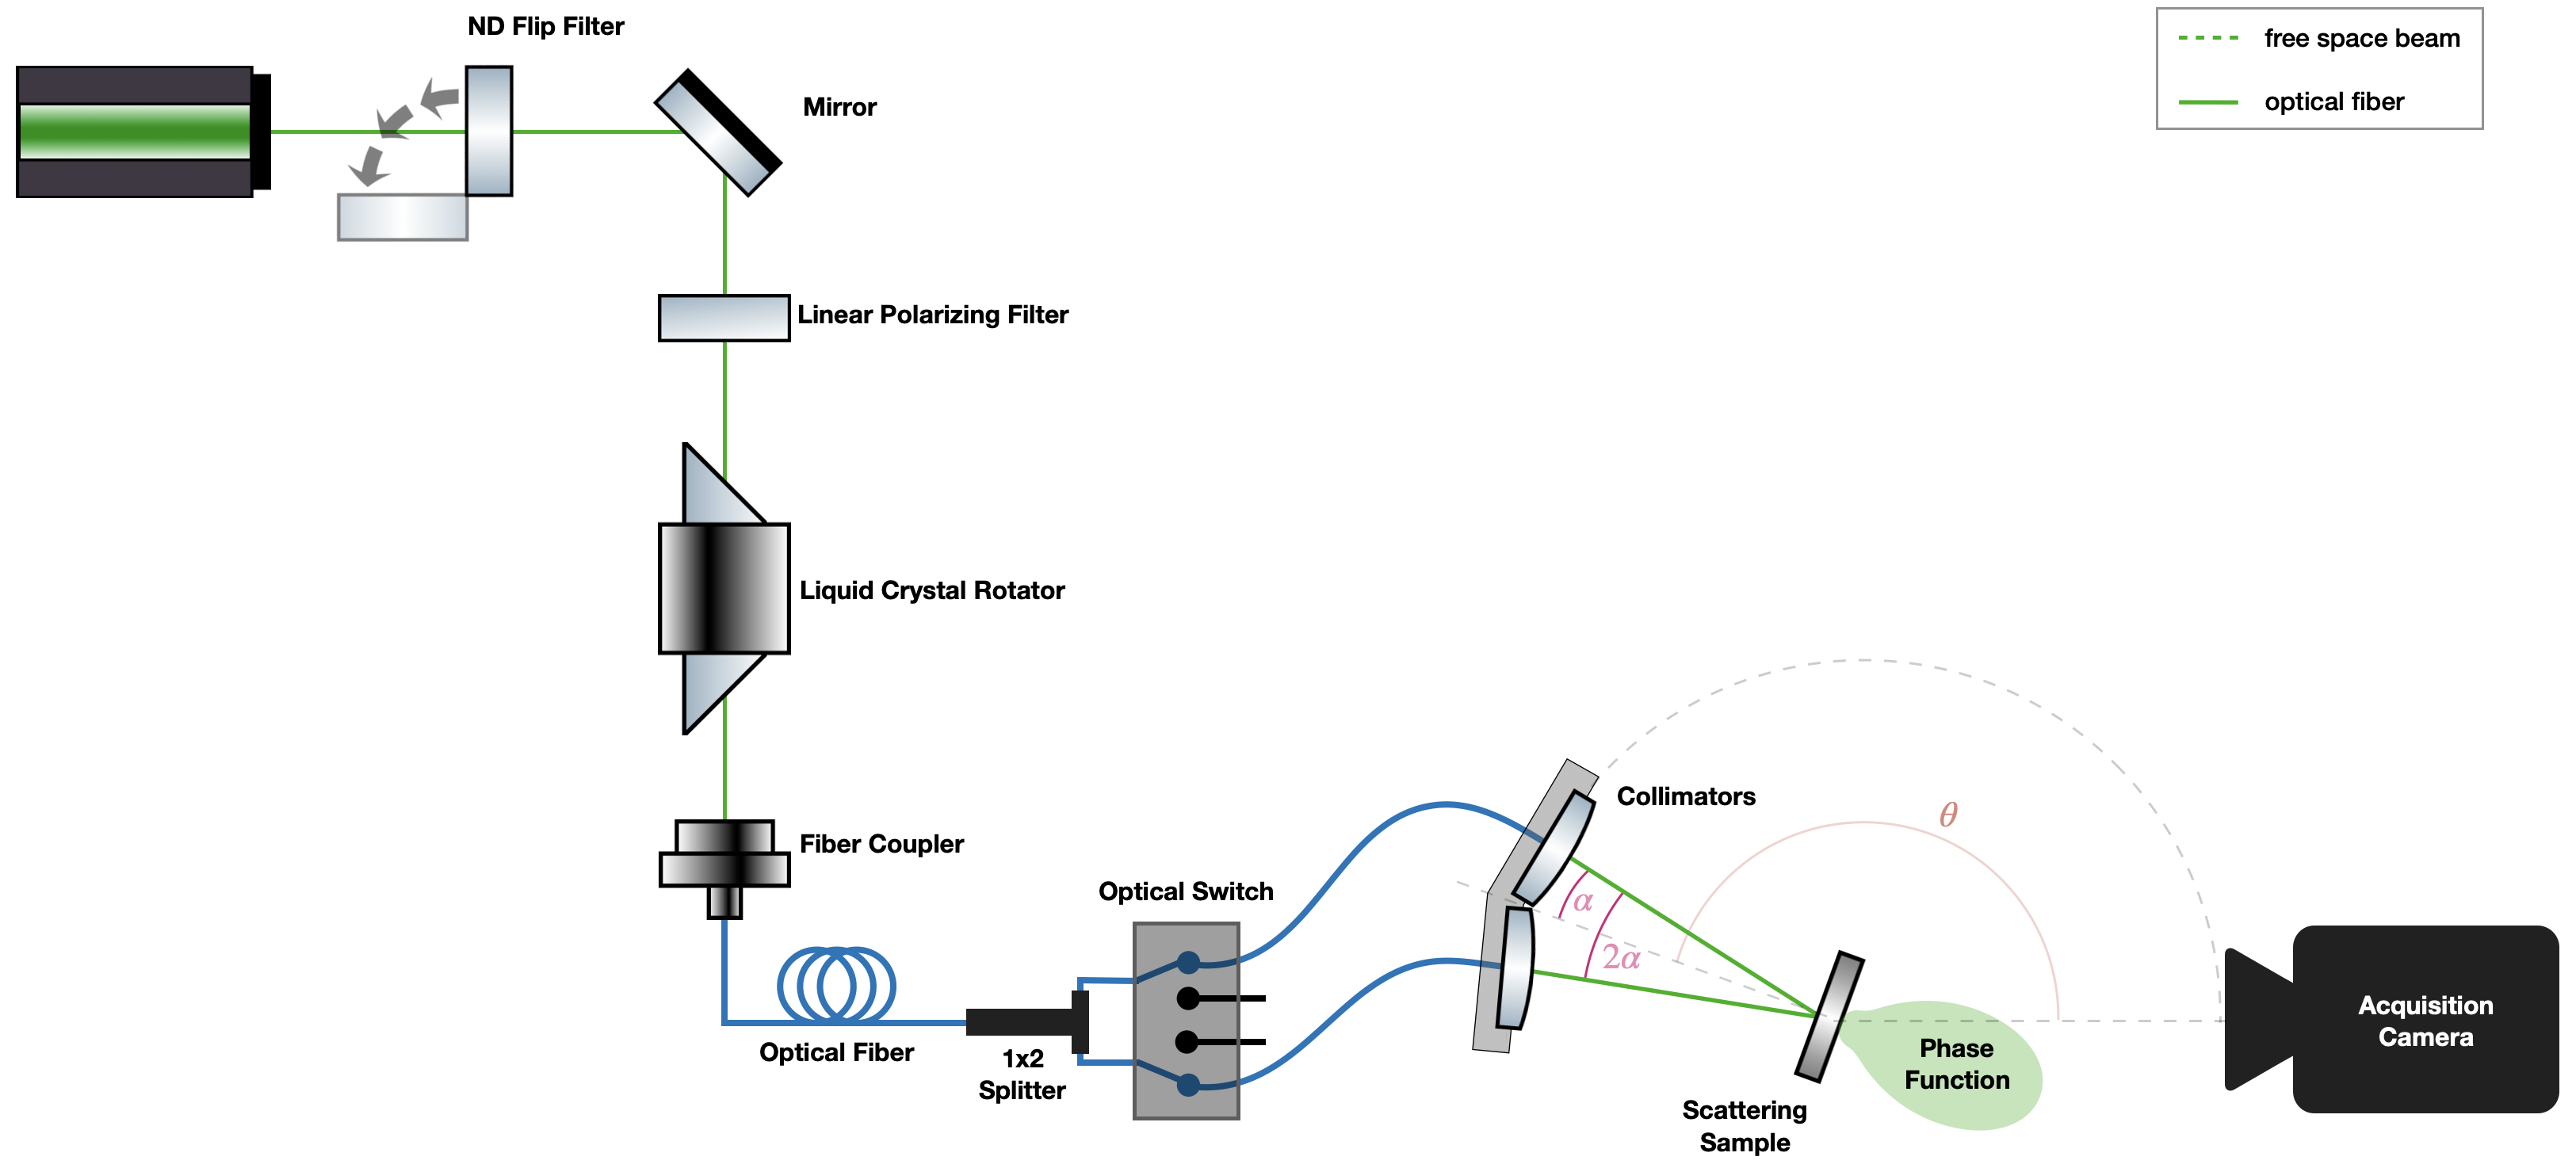
\includegraphics[width=0.75\textwidth]{design/figures/laser_path.png}
    \caption{Light path diagram for speckle correlation scatterometer}
    \label{fig:light_path}
\end{figure}

\subsection{Acquisition camera}
The acquisition camera must record high-contrast speckle images and assign directions to light arriving at the camera. A desirable camera and lens combination is one that maximizes angular resolution and light efficiency. Therefore, we choose a camera with a large sensor and small pixel pitch, and a fast lens focused at infinity with a long focal length.

\paragraph{Lens Focal Length} Computing the speckle correlation from images produced by the two illuminators requires both beams to fall within the camera's FOV. Since we maximize single-scattered light by minimizing the illuminator separation, a lens with a small FOV corresponds to illuminators with a small angular separation. However, due to the finite size of the kinematic mounts, there is a minimum vertical separation. This minimum vertical separation and the FOV-limited angle between the beams define a triangle whose length is the distance from the illuminators' kinematic mounts to the scattering sample. An 85 mm lens allows a small beam angle $2.47^\circ$ relative to horizontal and an overall setup size that complies with space constraints.

We use a FLIR Grasshopper scientific camera model GS3-PGE-91S6M-C with an AF-S Nikkor 85mm f/1.4G lens for acquisition.

\begin{table}[htbp]
    \renewcommand{\arraystretch}{1.25}
    \caption{Acquisition camera specifications}
    \begin{center}
        \begin{tabular}{ l l l l l }
        \toprule[2pt]
         \textbf{Property} & \textbf{Spec} \\
         \midrule[0.75pt]
         Camera Model & GS3-PGE-91S6M-C \\
         Resolution & $3376 \times 2704$ \\
         Megapixels & 9.1 \\
         Pitch & 3.69 $\mu$m \\
         Sensor & Sony ICX814 \\
         Sensor Type & CCD \\
         Sensor Size & $12 \times 10$ mm \\
         Spectrum & Mono \\
         Lens Make & Nikkor \\
         Lens Focal Length & 85 mm \\
         Lens Aperture & f/1.4 \\
         Lens Working Distance & $\infty$ \\
         \bottomrule[2pt]
        \end{tabular}
        \label{tab:acquisition_camera}
    \end{center}
\end{table}

\subsection{Illuminator assembly}
The illuminator motion assembly controls the illumination beams' directions both in azimuth and elevation. The primary design considerations are high angular resolution and repeatability for fine control of the illumination configuration, and structural stability to minimize vibrations. Each illuminator is attached to a 2-axis kinematic mount that allows $\pm 5^\circ$ in tip and  $\pm 3^\circ$ in tilt. Both kinematic mounts are attached to a custom collimator mount that minimizes their vertical separation while complying with the FOV constraint of $4.93^\circ$ between the illuminators. The collimator mount is attached to the azimuthal rotation stage via an aluminum extrusion.

\begin{figure}
    \centering
    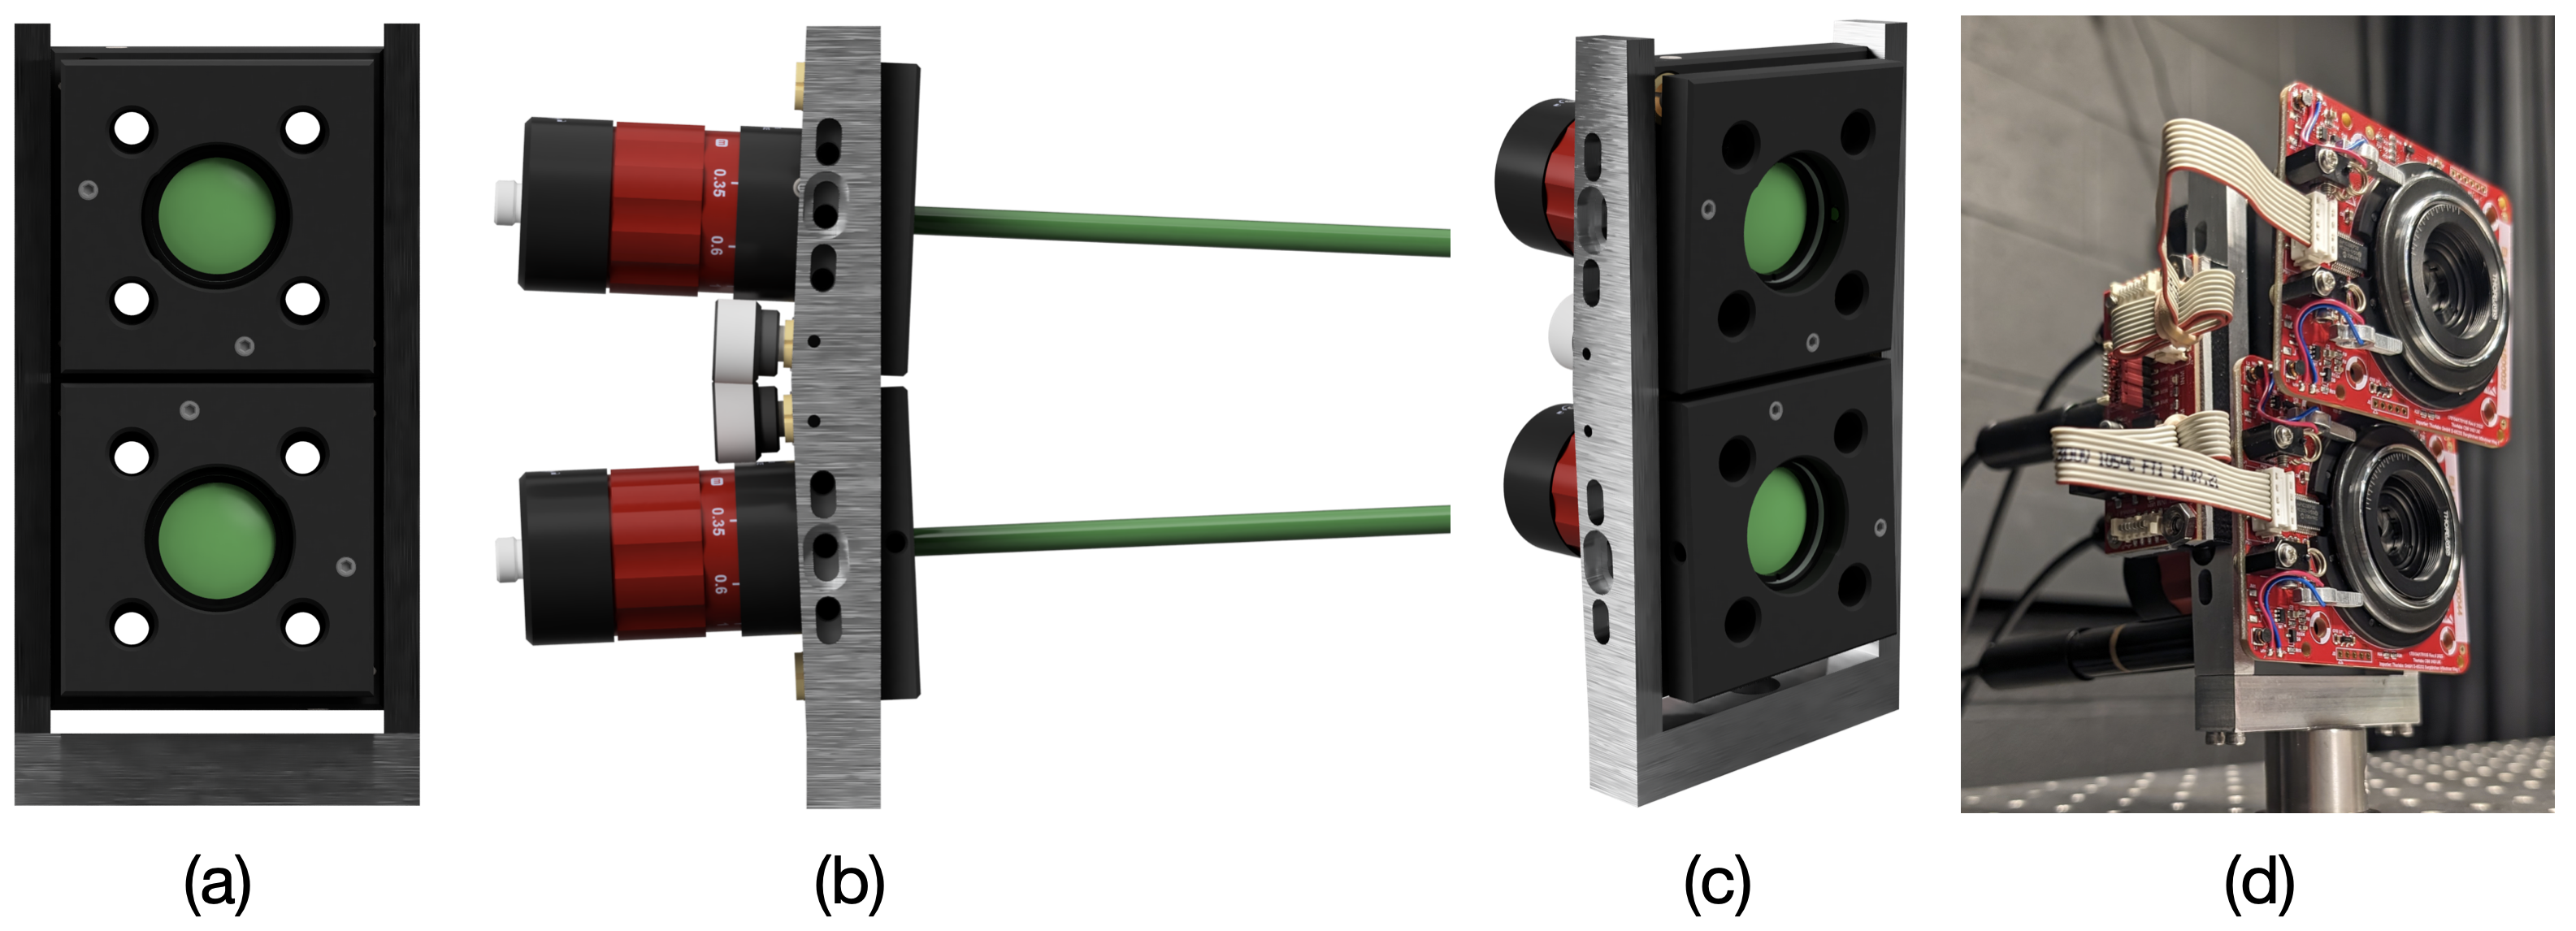
\includegraphics[width=\linewidth]{figures/collimator_assembly_summary.png}
    \caption{(a) CAD front view of collimator mount; (b) CAD side view showing the relative orientations of illumination beams; (c) CAD perspective view; (d) Fully assembled collimator mount which controls vertical and angular illuminator separation. Beam diameter is also controlled using motorized iris diaphragms.}
    \label{fig:collimator_mount}
\end{figure}

\subsection{Sample assembly}
The sample motion assembly is primarily used to rotate the scattering sample in order to maximize the amount of laser light transmitted through the air-glass interface as the illuminators' azimuthal position changes. This rotation is controlled by a small rotation stage which is mounted on an XYZ stage and an tip/tilt stage. These additional stages are used to control the rotation stage's orientation so it can made to be collinear with the illuminator assembly's azimuthal rotation axis. There is an additional translation stage mounted to the rotation stage's motion plate that is used to align the center of a mounted sample with the upper- and lower motion stages' rotation axes.
\begin{figure}
    \centering
    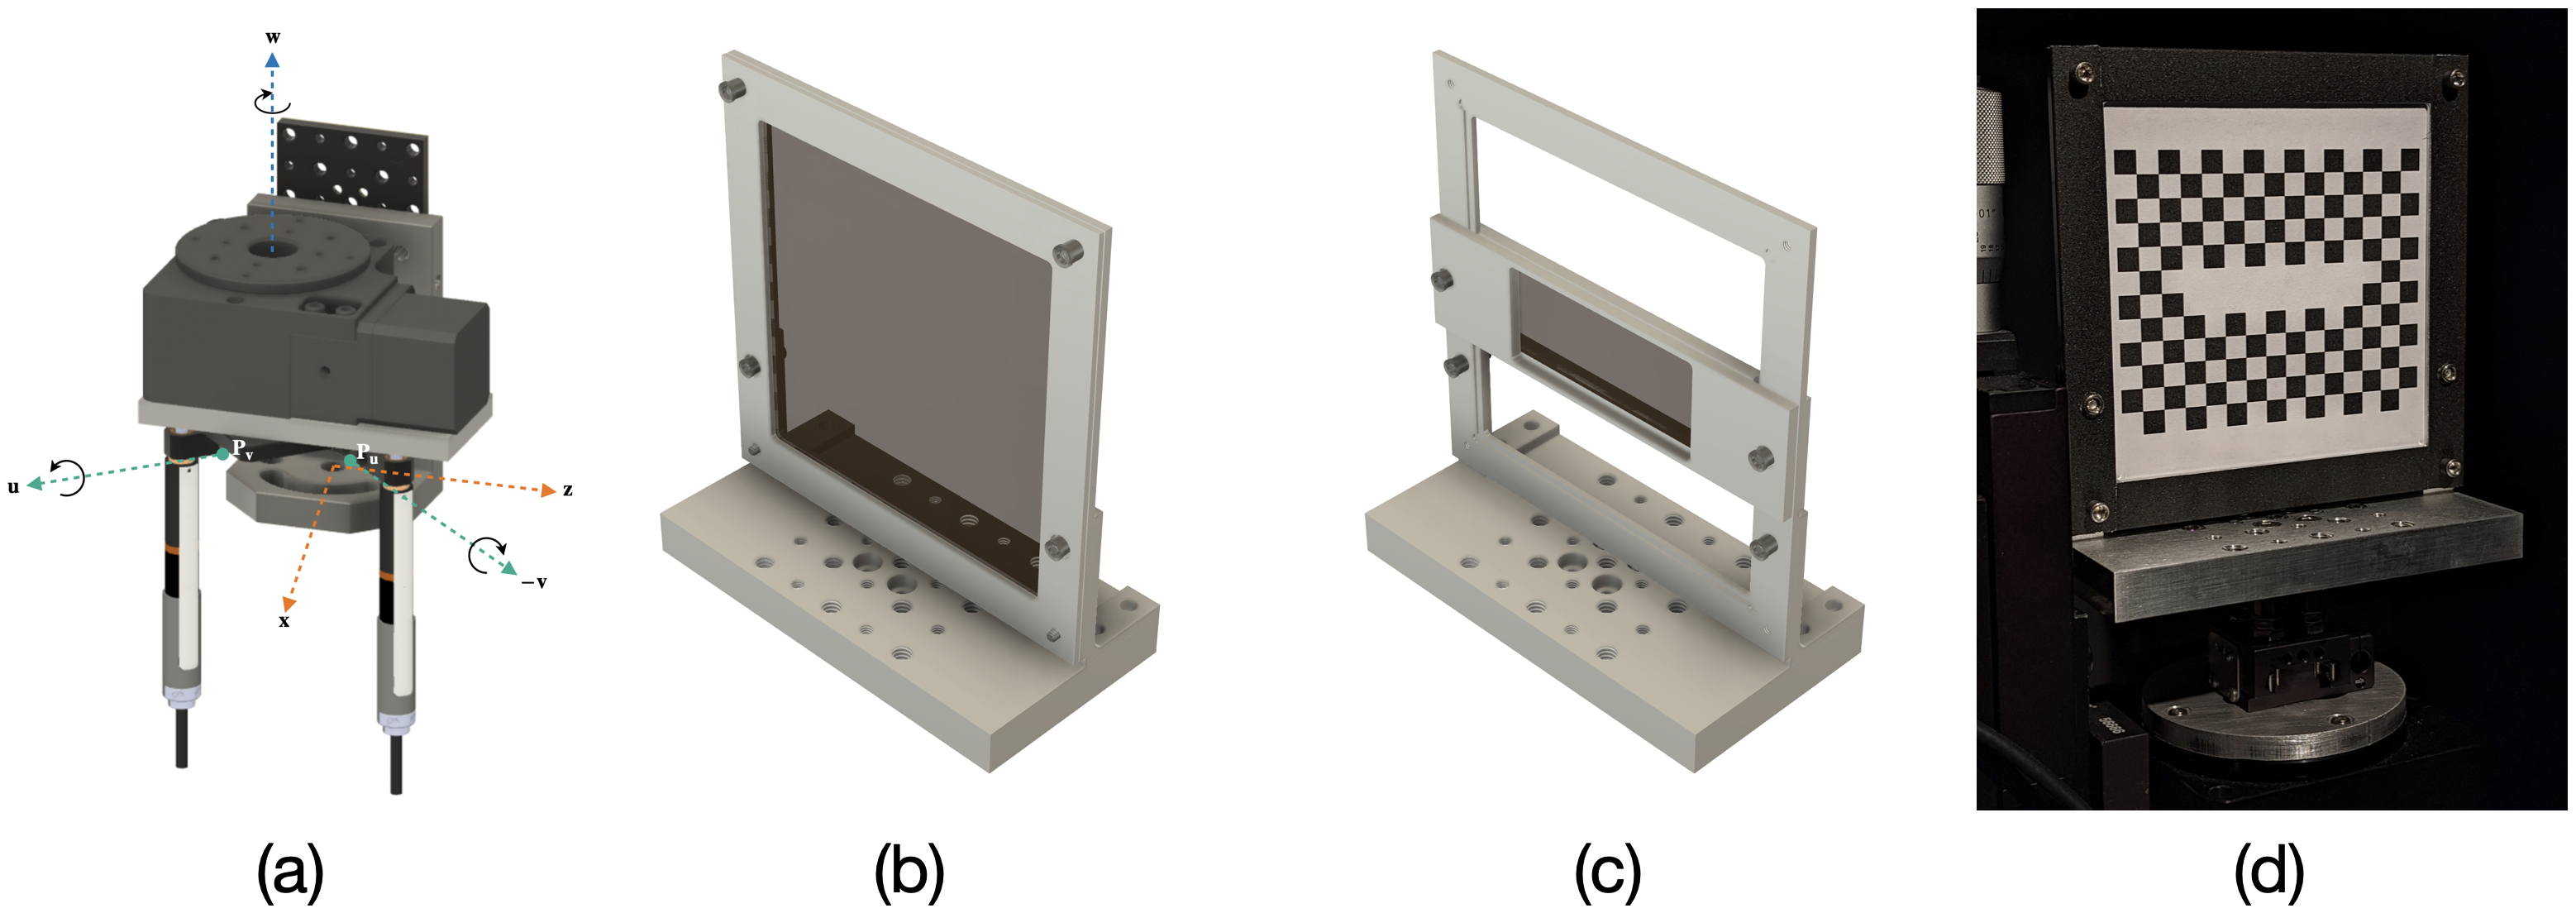
\includegraphics[width=\linewidth]{figures/sample_assembly_summary.png}
    \caption{(a) Sample motion assembly without sample mount; (b) Sample mount configured for calibration target (not drawn to scale with respect to (a)); (c) Sample mount configured for scattering sample on a microscope slide (not drawn to scale with respect to (a)); (d) Sample mount shown on top of sample assembly with calibration target installed}
    \label{fig:sample_motion_assy}
\end{figure}

\subsubsection{Sample Mount}
The sample mount is a custom, dual purpose mount used to hold scattering samples during acquisition and checkerboard targets during calibration. It is designed such that the front face of a calibration target is in the same plane as the central plane of a scattering sample. It consists of a base and angle mounts used to attach a square aluminum frame that holds a $10 \times 10$ cm glass window in place through compression by tightening four thumbscrews. Scattering samples are mounted by removing the aluminum frame's front face and attaching an inset frame that holds microscope slides via compression.